% Options for packages loaded elsewhere
\PassOptionsToPackage{unicode}{hyperref}
\PassOptionsToPackage{hyphens}{url}
\PassOptionsToPackage{dvipsnames,svgnames,x11names}{xcolor}
%
\documentclass[
  letterpaper,
  DIV=11,
  numbers=noendperiod]{scrreprt}

\usepackage{amsmath,amssymb}
\usepackage{iftex}
\ifPDFTeX
  \usepackage[T1]{fontenc}
  \usepackage[utf8]{inputenc}
  \usepackage{textcomp} % provide euro and other symbols
\else % if luatex or xetex
  \usepackage{unicode-math}
  \defaultfontfeatures{Scale=MatchLowercase}
  \defaultfontfeatures[\rmfamily]{Ligatures=TeX,Scale=1}
\fi
\usepackage{lmodern}
\ifPDFTeX\else  
    % xetex/luatex font selection
\fi
% Use upquote if available, for straight quotes in verbatim environments
\IfFileExists{upquote.sty}{\usepackage{upquote}}{}
\IfFileExists{microtype.sty}{% use microtype if available
  \usepackage[]{microtype}
  \UseMicrotypeSet[protrusion]{basicmath} % disable protrusion for tt fonts
}{}
\makeatletter
\@ifundefined{KOMAClassName}{% if non-KOMA class
  \IfFileExists{parskip.sty}{%
    \usepackage{parskip}
  }{% else
    \setlength{\parindent}{0pt}
    \setlength{\parskip}{6pt plus 2pt minus 1pt}}
}{% if KOMA class
  \KOMAoptions{parskip=half}}
\makeatother
\usepackage{xcolor}
\setlength{\emergencystretch}{3em} % prevent overfull lines
\setcounter{secnumdepth}{5}
% Make \paragraph and \subparagraph free-standing
\ifx\paragraph\undefined\else
  \let\oldparagraph\paragraph
  \renewcommand{\paragraph}[1]{\oldparagraph{#1}\mbox{}}
\fi
\ifx\subparagraph\undefined\else
  \let\oldsubparagraph\subparagraph
  \renewcommand{\subparagraph}[1]{\oldsubparagraph{#1}\mbox{}}
\fi

\usepackage{color}
\usepackage{fancyvrb}
\newcommand{\VerbBar}{|}
\newcommand{\VERB}{\Verb[commandchars=\\\{\}]}
\DefineVerbatimEnvironment{Highlighting}{Verbatim}{commandchars=\\\{\}}
% Add ',fontsize=\small' for more characters per line
\usepackage{framed}
\definecolor{shadecolor}{RGB}{241,243,245}
\newenvironment{Shaded}{\begin{snugshade}}{\end{snugshade}}
\newcommand{\AlertTok}[1]{\textcolor[rgb]{0.68,0.00,0.00}{#1}}
\newcommand{\AnnotationTok}[1]{\textcolor[rgb]{0.37,0.37,0.37}{#1}}
\newcommand{\AttributeTok}[1]{\textcolor[rgb]{0.40,0.45,0.13}{#1}}
\newcommand{\BaseNTok}[1]{\textcolor[rgb]{0.68,0.00,0.00}{#1}}
\newcommand{\BuiltInTok}[1]{\textcolor[rgb]{0.00,0.23,0.31}{#1}}
\newcommand{\CharTok}[1]{\textcolor[rgb]{0.13,0.47,0.30}{#1}}
\newcommand{\CommentTok}[1]{\textcolor[rgb]{0.37,0.37,0.37}{#1}}
\newcommand{\CommentVarTok}[1]{\textcolor[rgb]{0.37,0.37,0.37}{\textit{#1}}}
\newcommand{\ConstantTok}[1]{\textcolor[rgb]{0.56,0.35,0.01}{#1}}
\newcommand{\ControlFlowTok}[1]{\textcolor[rgb]{0.00,0.23,0.31}{#1}}
\newcommand{\DataTypeTok}[1]{\textcolor[rgb]{0.68,0.00,0.00}{#1}}
\newcommand{\DecValTok}[1]{\textcolor[rgb]{0.68,0.00,0.00}{#1}}
\newcommand{\DocumentationTok}[1]{\textcolor[rgb]{0.37,0.37,0.37}{\textit{#1}}}
\newcommand{\ErrorTok}[1]{\textcolor[rgb]{0.68,0.00,0.00}{#1}}
\newcommand{\ExtensionTok}[1]{\textcolor[rgb]{0.00,0.23,0.31}{#1}}
\newcommand{\FloatTok}[1]{\textcolor[rgb]{0.68,0.00,0.00}{#1}}
\newcommand{\FunctionTok}[1]{\textcolor[rgb]{0.28,0.35,0.67}{#1}}
\newcommand{\ImportTok}[1]{\textcolor[rgb]{0.00,0.46,0.62}{#1}}
\newcommand{\InformationTok}[1]{\textcolor[rgb]{0.37,0.37,0.37}{#1}}
\newcommand{\KeywordTok}[1]{\textcolor[rgb]{0.00,0.23,0.31}{#1}}
\newcommand{\NormalTok}[1]{\textcolor[rgb]{0.00,0.23,0.31}{#1}}
\newcommand{\OperatorTok}[1]{\textcolor[rgb]{0.37,0.37,0.37}{#1}}
\newcommand{\OtherTok}[1]{\textcolor[rgb]{0.00,0.23,0.31}{#1}}
\newcommand{\PreprocessorTok}[1]{\textcolor[rgb]{0.68,0.00,0.00}{#1}}
\newcommand{\RegionMarkerTok}[1]{\textcolor[rgb]{0.00,0.23,0.31}{#1}}
\newcommand{\SpecialCharTok}[1]{\textcolor[rgb]{0.37,0.37,0.37}{#1}}
\newcommand{\SpecialStringTok}[1]{\textcolor[rgb]{0.13,0.47,0.30}{#1}}
\newcommand{\StringTok}[1]{\textcolor[rgb]{0.13,0.47,0.30}{#1}}
\newcommand{\VariableTok}[1]{\textcolor[rgb]{0.07,0.07,0.07}{#1}}
\newcommand{\VerbatimStringTok}[1]{\textcolor[rgb]{0.13,0.47,0.30}{#1}}
\newcommand{\WarningTok}[1]{\textcolor[rgb]{0.37,0.37,0.37}{\textit{#1}}}

\providecommand{\tightlist}{%
  \setlength{\itemsep}{0pt}\setlength{\parskip}{0pt}}\usepackage{longtable,booktabs,array}
\usepackage{calc} % for calculating minipage widths
% Correct order of tables after \paragraph or \subparagraph
\usepackage{etoolbox}
\makeatletter
\patchcmd\longtable{\par}{\if@noskipsec\mbox{}\fi\par}{}{}
\makeatother
% Allow footnotes in longtable head/foot
\IfFileExists{footnotehyper.sty}{\usepackage{footnotehyper}}{\usepackage{footnote}}
\makesavenoteenv{longtable}
\usepackage{graphicx}
\makeatletter
\def\maxwidth{\ifdim\Gin@nat@width>\linewidth\linewidth\else\Gin@nat@width\fi}
\def\maxheight{\ifdim\Gin@nat@height>\textheight\textheight\else\Gin@nat@height\fi}
\makeatother
% Scale images if necessary, so that they will not overflow the page
% margins by default, and it is still possible to overwrite the defaults
% using explicit options in \includegraphics[width, height, ...]{}
\setkeys{Gin}{width=\maxwidth,height=\maxheight,keepaspectratio}
% Set default figure placement to htbp
\makeatletter
\def\fps@figure{htbp}
\makeatother
\newlength{\cslhangindent}
\setlength{\cslhangindent}{1.5em}
\newlength{\csllabelwidth}
\setlength{\csllabelwidth}{3em}
\newlength{\cslentryspacingunit} % times entry-spacing
\setlength{\cslentryspacingunit}{\parskip}
\newenvironment{CSLReferences}[2] % #1 hanging-ident, #2 entry spacing
 {% don't indent paragraphs
  \setlength{\parindent}{0pt}
  % turn on hanging indent if param 1 is 1
  \ifodd #1
  \let\oldpar\par
  \def\par{\hangindent=\cslhangindent\oldpar}
  \fi
  % set entry spacing
  \setlength{\parskip}{#2\cslentryspacingunit}
 }%
 {}
\usepackage{calc}
\newcommand{\CSLBlock}[1]{#1\hfill\break}
\newcommand{\CSLLeftMargin}[1]{\parbox[t]{\csllabelwidth}{#1}}
\newcommand{\CSLRightInline}[1]{\parbox[t]{\linewidth - \csllabelwidth}{#1}\break}
\newcommand{\CSLIndent}[1]{\hspace{\cslhangindent}#1}

\KOMAoption{captions}{tableheading}
\makeatletter
\makeatother
\makeatletter
\@ifpackageloaded{bookmark}{}{\usepackage{bookmark}}
\makeatother
\makeatletter
\@ifpackageloaded{caption}{}{\usepackage{caption}}
\AtBeginDocument{%
\ifdefined\contentsname
  \renewcommand*\contentsname{Table of contents}
\else
  \newcommand\contentsname{Table of contents}
\fi
\ifdefined\listfigurename
  \renewcommand*\listfigurename{List of Figures}
\else
  \newcommand\listfigurename{List of Figures}
\fi
\ifdefined\listtablename
  \renewcommand*\listtablename{List of Tables}
\else
  \newcommand\listtablename{List of Tables}
\fi
\ifdefined\figurename
  \renewcommand*\figurename{Figure}
\else
  \newcommand\figurename{Figure}
\fi
\ifdefined\tablename
  \renewcommand*\tablename{Table}
\else
  \newcommand\tablename{Table}
\fi
}
\@ifpackageloaded{float}{}{\usepackage{float}}
\floatstyle{ruled}
\@ifundefined{c@chapter}{\newfloat{codelisting}{h}{lop}}{\newfloat{codelisting}{h}{lop}[chapter]}
\floatname{codelisting}{Listing}
\newcommand*\listoflistings{\listof{codelisting}{List of Listings}}
\makeatother
\makeatletter
\@ifpackageloaded{caption}{}{\usepackage{caption}}
\@ifpackageloaded{subcaption}{}{\usepackage{subcaption}}
\makeatother
\makeatletter
\@ifpackageloaded{tcolorbox}{}{\usepackage[skins,breakable]{tcolorbox}}
\makeatother
\makeatletter
\@ifundefined{shadecolor}{\definecolor{shadecolor}{rgb}{.97, .97, .97}}
\makeatother
\makeatletter
\makeatother
\makeatletter
\makeatother
\ifLuaTeX
  \usepackage{selnolig}  % disable illegal ligatures
\fi
\IfFileExists{bookmark.sty}{\usepackage{bookmark}}{\usepackage{hyperref}}
\IfFileExists{xurl.sty}{\usepackage{xurl}}{} % add URL line breaks if available
\urlstyle{same} % disable monospaced font for URLs
\hypersetup{
  pdftitle={Manual-Applied-Spatial-Ecology},
  pdfauthor={W. David Walter},
  colorlinks=true,
  linkcolor={blue},
  filecolor={Maroon},
  citecolor={Blue},
  urlcolor={Blue},
  pdfcreator={LaTeX via pandoc}}

\title{Manual-Applied-Spatial-Ecology}
\author{W. David Walter}
\date{2023-12-11}

\begin{document}
\maketitle
\ifdefined\Shaded\renewenvironment{Shaded}{\begin{tcolorbox}[boxrule=0pt, sharp corners, frame hidden, enhanced, borderline west={3pt}{0pt}{shadecolor}, interior hidden, breakable]}{\end{tcolorbox}}\fi

\renewcommand*\contentsname{Table of contents}
{
\hypersetup{linkcolor=}
\setcounter{tocdepth}{2}
\tableofcontents
}
\# {[}Preface{]}(--- title: ``Manual of Applied Spatial Ecology''author:
``W. David Walter''date: ``r Sys.Date()''site:
bookdown::bookdown\_siteoutput: bookdown::pdf\_book
\#bookdown::gitbookdocumentclass: bookbibliography: {[}book.bib,
packages.bib{]}biblio-style: apalikelink-citations: yescolorlinks:
yes\#github-repo: rstudio/bookdown-demodescription: ``Final version of
manual prior to conversion to terra and sf packages''\#graphics:
yes\#cover-image: ``CoverSlide2.jpg''header-includes: -

\usepackage{titling}

\pretitle{\begin{center}    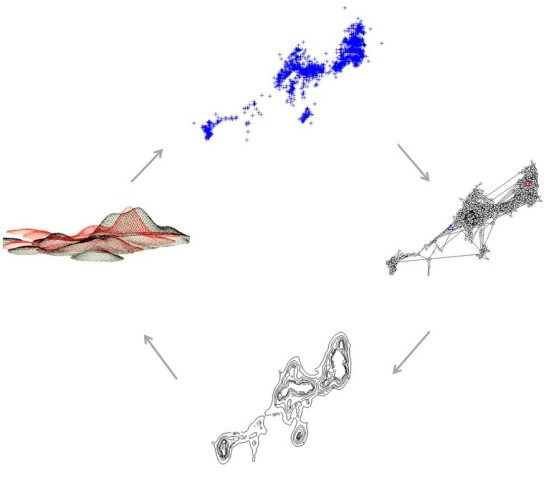
\includegraphics[width=2in,height=2in]{CoverSlide2.jpg}\LARGE\\}
- \posttitle{\end{center}}---\mainmatter\# Preface \{-\}The purpose of
this manual is to assist researchers on methods for data management and
analysisusing the R environment or other software after data has been
collected in the field. The impetusbehind this manual was from many
years of frustration in trying to analyze data in R usingcode and
forgetting how it was done upon completion of a study. We wanted to find
a way toavoid needing to search computers for folders to find old R code
then try to remember what wedid to the data to get the code to run
properly. Over the years, advancements in data handlingand manipulation,
GIS capabilities, and methods of estimators for home range,
movements,resource selection, and spatial epidemiology have occurred
within the R environment. ProgramR is free and used by researchers
world-wide but R also provides a platform to create and displayspatial
layers without the need for the variety of GUI software, free or
otherwise. Furthermore,analyzing spatial data in R enables statistical
analysis of data without the errors that may arisefrom bringing data
from spreadsheet or GIS software to statistical programs.We would like
to stress that this manual is not the authority on all topics presented
herein.Our goal was to create an online manual that could be easily
followed by researchers, biologists,or graduate students to analyze
their data in R. Although the user would benefit from
generalintroductory knowledge of using R and ArcMap, most of the manual
is for mid-level users ofR that need guidance beyond the basics of
introductory R and GIS coureses. We also providenumerous citations
throughout each section should the user choose to learn the theory or
moredetails behind each topic. In addition, this manual provides a handy
outline of course materialsfor an Applied Spatial Ecology course that
will surely expand or change as the field evolves. Astime permits and
errors are brought to our attention, we plan to update and correct
problemsso be sure to send any corrections or comments our way.Any use
of trade, firm, or product names is for descriptive purposes only and
does not implyendorsement by the U.S. Government.Recommended
citation:Walter, W.D. Manual of Applied Spatial Ecology. Walter Applied
SpatialEcology Lab, Pennsylvania State University, University Park.
Access
Date.http://ecosystems.psu.edu/research/labs/walter-lab.\newpage**Acknowledgments**Numerous
colleagues have provide assistance with R packages they created or with
code theyhave provided in some other form. We would be remiss if we
failed to thank these colleaguesfor their hard work:Sharon Baruch-Mordo,
The Nature Conservancy, Fort Collins, CO 80524 ;
sbaruch-mordo@tnc.orgSimon Benhamou, Centre d'Ecologie Fonctionnelle et
Evolutive, FranceClément Calenge, Data Analysis Support Unit,
Directorate for Studies and Research, NationalOffice of Hunting and Wild
Fauna, Saint Benoist - 78610 Auffargis, FranceMevin Hooten, Colorado
Cooperative Fish and Wildlife Research Unit, 201 Wagar Bldg,
ColoradoState University, Fort Collins, CO 8052 ;
Mevin.Hooten@colostate.eduBill Kanapaux, Pennsylvania Cooperative Fish
and Wildlife Research Unit, 406 Forest ResourcesBldg., Pennyslvania
State University, University Park, PA 16802 ; wjk15@psu.eduBart
Kranstauber, Max Planck Institute for Ornithology,
Eberhard-Gwinner-Str., 82319
Seewiesen;bart.kranstauber@uni-konstanz.deRyan Nielsen, West Inc.,415 W.
17th St.~Suite 200, Cheyenne, WY 82001 ; rnielson@westinc.comGlen
Sargeant, Northern Prairie Wildlife Research Center, Jamestown, North
Dakota;glen\_sargeant@usgs.govPeter Singleton, USDA Forest Service,
Pacific Northwest Research Station in Wenatchee,
WA;singlep@u.washington.eduMarcó Smolla, Max Planck Institute for
Ornithology, Dept. Migration and Immuno-ecology,Am Obstberg 1, 78315
Radolfzell, Germany; msmolla@orn.mpg.deTyler Wagner, US Geological
Survey, Pennsylvania Cooperative Fish and Wildlife ResearchUnit, 402
Forest Resources Bldg., Pennsylvania State University, University Park,
PA 16802 ;twagner@psu.edu) \{.unnumbered\}

\bookmarksetup{startatroot}

\hypertarget{the-purpose-of-this-manual-is-to-assist-researchers-on-methods-for-data-management-and-analysisusing-the-r-environment-or-other-software-after-data-has-been-collected-in-the-field.-the-impetusbehind-this-manual-was-from-many-years-of-frustration-in-trying-to-analyze-data-in-r-usingcode-and-forgetting-how-it-was-done-upon-completion-of-a-study.-we-wanted-to-find-a-way-toavoid-needing-to-search-computers-for-folders-to-find-old-r-code-then-try-to-remember-what-wedid-to-the-data-to-get-the-code-to-run-properly.-over-the-years-advancements-in-data-handlingand-manipulation-gis-capabilities-and-methods-of-estimators-for-home-range-movementsresource-selection-and-spatial-epidemiology-have-occurred-within-the-r-environment.-programr-is-free-and-used-by-researchers-world-wide-but-r-also-provides-a-platform-to-create-and-displayspatial-layers-without-the-need-for-the-variety-of-gui-software-free-or-otherwise.-furthermoreanalyzing-spatial-data-in-r-enables-statistical-analysis-of-data-without-the-errors-that-may-arisefrom-bringing-data-from-spreadsheet-or-gis-software-to-statistical-programs.we-would-like-to-stress-that-this-manual-is-not-the-authority-on-all-topics-presented-herein.our-goal-was-to-create-an-online-manual-that-could-be-easily-followed-by-researchers-biologistsor-graduate-students-to-analyze-their-data-in-r.-although-the-user-would-benefit-from-generalintroductory-knowledge-of-using-r-and-arcmap-most-of-the-manual-is-for-mid-level-users-ofr-that-need-guidance-beyond-the-basics-of-introductory-r-and-gis-coureses.-we-also-providenumerous-citations-throughout-each-section-should-the-user-choose-to-learn-the-theory-or-moredetails-behind-each-topic.-in-addition-this-manual-provides-a-handy-outline-of-course-materialsfor-an-applied-spatial-ecology-course-that-will-surely-expand-or-change-as-the-field-evolves.-astime-permits-and-errors-are-brought-to-our-attention-we-plan-to-update-and-correct-problemsso-be-sure-to-send-any-corrections-or-comments-our-way.any-use-of-trade-firm-or-product-names-is-for-descriptive-purposes-only-and-does-not-implyendorsement-by-the-u.s.-government.recommended-citationwalter-w.d.-manual-of-applied-spatial-ecology.-walter-applied-spatialecology-lab-pennsylvania-state-university-university-park.-access-date.httpecosystems.psu.eduresearchlabswalter-lab.acknowledgmentsnumerous-colleagues-have-provide-assistance-with-r-packages-they-created-or-with-code-theyhave-provided-in-some-other-form.-we-would-be-remiss-if-we-failed-to-thank-these-colleaguesfor-their-hard-worksharon-baruch-mordo-the-nature-conservancy-fort-collins-co-80524-sbaruch-mordotnc.orgsimon-benhamou-centre-decologie-fonctionnelle-et-evolutive-francecluxe9ment-calenge-data-analysis-support-unit-directorate-for-studies-and-research-nationaloffice-of-hunting-and-wild-fauna-saint-benoist---78610-auffargis-francemevin-hooten-colorado-cooperative-fish-and-wildlife-research-unit-201-wagar-bldg-coloradostate-university-fort-collins-co-8052-mevin.hootencolostate.edubill-kanapaux-pennsylvania-cooperative-fish-and-wildlife-research-unit-406-forest-resourcesbldg.-pennyslvania-state-university-university-park-pa-16802-wjk15psu.edubart-kranstauber-max-planck-institute-for-ornithology-eberhard-gwinner-str.-82319-seewiesenbart.kranstauberuni-konstanz.deryan-nielsen-west-inc.415-w.-17th-st.-suite-200-cheyenne-wy-82001-rnielsonwestinc.comglen-sargeant-northern-prairie-wildlife-research-center-jamestown-north-dakotaglen_sargeantusgs.govpeter-singleton-usda-forest-service-pacific-northwest-research-station-in-wenatchee-wasinglepu.washington.edumarcuxf3-smolla-max-planck-institute-for-ornithology-dept.-migration-and-immuno-ecologyam-obstberg-1-78315-radolfzell-germany-msmollaorn.mpg.detyler-wagner-us-geological-survey-pennsylvania-cooperative-fish-and-wildlife-researchunit-402-forest-resources-bldg.-pennsylvania-state-university-university-park-pa-16802-twagnerpsu.edu}{%
\chapter*{\texorpdfstring{The purpose of this manual is to assist
researchers on methods for data management and analysisusing the R
environment or other software after data has been collected in the
field. The impetusbehind this manual was from many years of frustration
in trying to analyze data in R usingcode and forgetting how it was done
upon completion of a study. We wanted to find a way toavoid needing to
search computers for folders to find old R code then try to remember
what wedid to the data to get the code to run properly. Over the years,
advancements in data handlingand manipulation, GIS capabilities, and
methods of estimators for home range, movements,resource selection, and
spatial epidemiology have occurred within the R environment. ProgramR is
free and used by researchers world-wide but R also provides a platform
to create and displayspatial layers without the need for the variety of
GUI software, free or otherwise. Furthermore,analyzing spatial data in R
enables statistical analysis of data without the errors that may
arisefrom bringing data from spreadsheet or GIS software to statistical
programs.We would like to stress that this manual is not the authority
on all topics presented herein.Our goal was to create an online manual
that could be easily followed by researchers, biologists,or graduate
students to analyze their data in R. Although the user would benefit
from generalintroductory knowledge of using R and ArcMap, most of the
manual is for mid-level users ofR that need guidance beyond the basics
of introductory R and GIS coureses. We also providenumerous citations
throughout each section should the user choose to learn the theory or
moredetails behind each topic. In addition, this manual provides a handy
outline of course materialsfor an Applied Spatial Ecology course that
will surely expand or change as the field evolves. Astime permits and
errors are brought to our attention, we plan to update and correct
problemsso be sure to send any corrections or comments our way.Any use
of trade, firm, or product names is for descriptive purposes only and
does not implyendorsement by the U.S. Government.\textbf{Recommended
citation}:Walter, W.D. Manual of Applied Spatial Ecology. Walter Applied
SpatialEcology Lab, Pennsylvania State University, University Park.
Access
Date.\url{http://ecosystems.psu.edu/research/labs/walter-lab}.\newpage**Acknowledgments**Numerous
colleagues have provide assistance with R packages they created or with
code theyhave provided in some other form. We would be remiss if we
failed to thank these colleaguesfor their hard work:Sharon Baruch-Mordo,
The Nature Conservancy, Fort Collins, CO 80524 ;
sbaruch-mordo@tnc.orgSimon Benhamou, Centre d'Ecologie Fonctionnelle et
Evolutive, FranceClément Calenge, Data Analysis Support Unit,
Directorate for Studies and Research, NationalOffice of Hunting and Wild
Fauna, Saint Benoist - 78610 Auffargis, FranceMevin Hooten, Colorado
Cooperative Fish and Wildlife Research Unit, 201 Wagar Bldg,
ColoradoState University, Fort Collins, CO 8052 ;
Mevin.Hooten@colostate.eduBill Kanapaux, Pennsylvania Cooperative Fish
and Wildlife Research Unit, 406 Forest ResourcesBldg., Pennyslvania
State University, University Park, PA 16802 ; wjk15@psu.eduBart
Kranstauber, Max Planck Institute for Ornithology,
Eberhard-Gwinner-Str., 82319
Seewiesen;bart.kranstauber@uni-konstanz.deRyan Nielsen, West Inc.,415 W.
17th St.~Suite 200, Cheyenne, WY 82001 ; rnielson@westinc.comGlen
Sargeant, Northern Prairie Wildlife Research Center, Jamestown, North
Dakota;glen\_sargeant@usgs.govPeter Singleton, USDA Forest Service,
Pacific Northwest Research Station in Wenatchee,
WA;singlep@u.washington.eduMarcó Smolla, Max Planck Institute for
Ornithology, Dept. Migration and Immuno-ecology,Am Obstberg 1, 78315
Radolfzell, Germany; msmolla@orn.mpg.deTyler Wagner, US Geological
Survey, Pennsylvania Cooperative Fish and Wildlife ResearchUnit, 402
Forest Resources Bldg., Pennsylvania State University, University Park,
PA 16802
;twagner@psu.edu}{The purpose of this manual is to assist researchers on methods for data management and analysisusing the R environment or other software after data has been collected in the field. The impetusbehind this manual was from many years of frustration in trying to analyze data in R usingcode and forgetting how it was done upon completion of a study. We wanted to find a way toavoid needing to search computers for folders to find old R code then try to remember what wedid to the data to get the code to run properly. Over the years, advancements in data handlingand manipulation, GIS capabilities, and methods of estimators for home range, movements,resource selection, and spatial epidemiology have occurred within the R environment. ProgramR is free and used by researchers world-wide but R also provides a platform to create and displayspatial layers without the need for the variety of GUI software, free or otherwise. Furthermore,analyzing spatial data in R enables statistical analysis of data without the errors that may arisefrom bringing data from spreadsheet or GIS software to statistical programs.We would like to stress that this manual is not the authority on all topics presented herein.Our goal was to create an online manual that could be easily followed by researchers, biologists,or graduate students to analyze their data in R. Although the user would benefit from generalintroductory knowledge of using R and ArcMap, most of the manual is for mid-level users ofR that need guidance beyond the basics of introductory R and GIS coureses. We also providenumerous citations throughout each section should the user choose to learn the theory or moredetails behind each topic. In addition, this manual provides a handy outline of course materialsfor an Applied Spatial Ecology course that will surely expand or change as the field evolves. Astime permits and errors are brought to our attention, we plan to update and correct problemsso be sure to send any corrections or comments our way.Any use of trade, firm, or product names is for descriptive purposes only and does not implyendorsement by the U.S. Government.Recommended citation:Walter, W.D. Manual of Applied Spatial Ecology. Walter Applied SpatialEcology Lab, Pennsylvania State University, University Park. Access Date.http://ecosystems.psu.edu/research/labs/walter-lab.**Acknowledgments**Numerous colleagues have provide assistance with R packages they created or with code theyhave provided in some other form. We would be remiss if we failed to thank these colleaguesfor their hard work:Sharon Baruch-Mordo, The Nature Conservancy, Fort Collins, CO 80524 ; sbaruch-mordo@tnc.orgSimon Benhamou, Centre d'Ecologie Fonctionnelle et Evolutive, FranceClément Calenge, Data Analysis Support Unit, Directorate for Studies and Research, NationalOffice of Hunting and Wild Fauna, Saint Benoist - 78610 Auffargis, FranceMevin Hooten, Colorado Cooperative Fish and Wildlife Research Unit, 201 Wagar Bldg, ColoradoState University, Fort Collins, CO 8052 ; Mevin.Hooten@colostate.eduBill Kanapaux, Pennsylvania Cooperative Fish and Wildlife Research Unit, 406 Forest ResourcesBldg., Pennyslvania State University, University Park, PA 16802 ; wjk15@psu.eduBart Kranstauber, Max Planck Institute for Ornithology, Eberhard-Gwinner-Str., 82319 Seewiesen;bart.kranstauber@uni-konstanz.deRyan Nielsen, West Inc.,415 W. 17th St.~Suite 200, Cheyenne, WY 82001 ; rnielson@westinc.comGlen Sargeant, Northern Prairie Wildlife Research Center, Jamestown, North Dakota;glen\_sargeant@usgs.govPeter Singleton, USDA Forest Service, Pacific Northwest Research Station in Wenatchee, WA;singlep@u.washington.eduMarcó Smolla, Max Planck Institute for Ornithology, Dept. Migration and Immuno-ecology,Am Obstberg 1, 78315 Radolfzell, Germany; msmolla@orn.mpg.deTyler Wagner, US Geological Survey, Pennsylvania Cooperative Fish and Wildlife ResearchUnit, 402 Forest Resources Bldg., Pennsylvania State University, University Park, PA 16802 ;twagner@psu.edu}}\label{the-purpose-of-this-manual-is-to-assist-researchers-on-methods-for-data-management-and-analysisusing-the-r-environment-or-other-software-after-data-has-been-collected-in-the-field.-the-impetusbehind-this-manual-was-from-many-years-of-frustration-in-trying-to-analyze-data-in-r-usingcode-and-forgetting-how-it-was-done-upon-completion-of-a-study.-we-wanted-to-find-a-way-toavoid-needing-to-search-computers-for-folders-to-find-old-r-code-then-try-to-remember-what-wedid-to-the-data-to-get-the-code-to-run-properly.-over-the-years-advancements-in-data-handlingand-manipulation-gis-capabilities-and-methods-of-estimators-for-home-range-movementsresource-selection-and-spatial-epidemiology-have-occurred-within-the-r-environment.-programr-is-free-and-used-by-researchers-world-wide-but-r-also-provides-a-platform-to-create-and-displayspatial-layers-without-the-need-for-the-variety-of-gui-software-free-or-otherwise.-furthermoreanalyzing-spatial-data-in-r-enables-statistical-analysis-of-data-without-the-errors-that-may-arisefrom-bringing-data-from-spreadsheet-or-gis-software-to-statistical-programs.we-would-like-to-stress-that-this-manual-is-not-the-authority-on-all-topics-presented-herein.our-goal-was-to-create-an-online-manual-that-could-be-easily-followed-by-researchers-biologistsor-graduate-students-to-analyze-their-data-in-r.-although-the-user-would-benefit-from-generalintroductory-knowledge-of-using-r-and-arcmap-most-of-the-manual-is-for-mid-level-users-ofr-that-need-guidance-beyond-the-basics-of-introductory-r-and-gis-coureses.-we-also-providenumerous-citations-throughout-each-section-should-the-user-choose-to-learn-the-theory-or-moredetails-behind-each-topic.-in-addition-this-manual-provides-a-handy-outline-of-course-materialsfor-an-applied-spatial-ecology-course-that-will-surely-expand-or-change-as-the-field-evolves.-astime-permits-and-errors-are-brought-to-our-attention-we-plan-to-update-and-correct-problemsso-be-sure-to-send-any-corrections-or-comments-our-way.any-use-of-trade-firm-or-product-names-is-for-descriptive-purposes-only-and-does-not-implyendorsement-by-the-u.s.-government.recommended-citationwalter-w.d.-manual-of-applied-spatial-ecology.-walter-applied-spatialecology-lab-pennsylvania-state-university-university-park.-access-date.httpecosystems.psu.eduresearchlabswalter-lab.acknowledgmentsnumerous-colleagues-have-provide-assistance-with-r-packages-they-created-or-with-code-theyhave-provided-in-some-other-form.-we-would-be-remiss-if-we-failed-to-thank-these-colleaguesfor-their-hard-worksharon-baruch-mordo-the-nature-conservancy-fort-collins-co-80524-sbaruch-mordotnc.orgsimon-benhamou-centre-decologie-fonctionnelle-et-evolutive-francecluxe9ment-calenge-data-analysis-support-unit-directorate-for-studies-and-research-nationaloffice-of-hunting-and-wild-fauna-saint-benoist---78610-auffargis-francemevin-hooten-colorado-cooperative-fish-and-wildlife-research-unit-201-wagar-bldg-coloradostate-university-fort-collins-co-8052-mevin.hootencolostate.edubill-kanapaux-pennsylvania-cooperative-fish-and-wildlife-research-unit-406-forest-resourcesbldg.-pennyslvania-state-university-university-park-pa-16802-wjk15psu.edubart-kranstauber-max-planck-institute-for-ornithology-eberhard-gwinner-str.-82319-seewiesenbart.kranstauberuni-konstanz.deryan-nielsen-west-inc.415-w.-17th-st.-suite-200-cheyenne-wy-82001-rnielsonwestinc.comglen-sargeant-northern-prairie-wildlife-research-center-jamestown-north-dakotaglen_sargeantusgs.govpeter-singleton-usda-forest-service-pacific-northwest-research-station-in-wenatchee-wasinglepu.washington.edumarcuxf3-smolla-max-planck-institute-for-ornithology-dept.-migration-and-immuno-ecologyam-obstberg-1-78315-radolfzell-germany-msmollaorn.mpg.detyler-wagner-us-geological-survey-pennsylvania-cooperative-fish-and-wildlife-researchunit-402-forest-resources-bldg.-pennsylvania-state-university-university-park-pa-16802-twagnerpsu.edu}}
\addcontentsline{toc}{chapter}{The purpose of this manual is to assist
researchers on methods for data management and analysisusing the R
environment or other software after data has been collected in the
field. The impetusbehind this manual was from many years of frustration
in trying to analyze data in R usingcode and forgetting how it was done
upon completion of a study. We wanted to find a way toavoid needing to
search computers for folders to find old R code then try to remember
what wedid to the data to get the code to run properly. Over the years,
advancements in data handlingand manipulation, GIS capabilities, and
methods of estimators for home range, movements,resource selection, and
spatial epidemiology have occurred within the R environment. ProgramR is
free and used by researchers world-wide but R also provides a platform
to create and displayspatial layers without the need for the variety of
GUI software, free or otherwise. Furthermore,analyzing spatial data in R
enables statistical analysis of data without the errors that may
arisefrom bringing data from spreadsheet or GIS software to statistical
programs.We would like to stress that this manual is not the authority
on all topics presented herein.Our goal was to create an online manual
that could be easily followed by researchers, biologists,or graduate
students to analyze their data in R. Although the user would benefit
from generalintroductory knowledge of using R and ArcMap, most of the
manual is for mid-level users ofR that need guidance beyond the basics
of introductory R and GIS coureses. We also providenumerous citations
throughout each section should the user choose to learn the theory or
moredetails behind each topic. In addition, this manual provides a handy
outline of course materialsfor an Applied Spatial Ecology course that
will surely expand or change as the field evolves. Astime permits and
errors are brought to our attention, we plan to update and correct
problemsso be sure to send any corrections or comments our way.Any use
of trade, firm, or product names is for descriptive purposes only and
does not implyendorsement by the U.S. Government.\textbf{Recommended
citation}:Walter, W.D. Manual of Applied Spatial Ecology. Walter Applied
SpatialEcology Lab, Pennsylvania State University, University Park.
Access
Date.\url{http://ecosystems.psu.edu/research/labs/walter-lab}.\newpage**Acknowledgments**Numerous
colleagues have provide assistance with R packages they created or with
code theyhave provided in some other form. We would be remiss if we
failed to thank these colleaguesfor their hard work:Sharon Baruch-Mordo,
The Nature Conservancy, Fort Collins, CO 80524 ;
sbaruch-mordo@tnc.orgSimon Benhamou, Centre d'Ecologie Fonctionnelle et
Evolutive, FranceClément Calenge, Data Analysis Support Unit,
Directorate for Studies and Research, NationalOffice of Hunting and Wild
Fauna, Saint Benoist - 78610 Auffargis, FranceMevin Hooten, Colorado
Cooperative Fish and Wildlife Research Unit, 201 Wagar Bldg,
ColoradoState University, Fort Collins, CO 8052 ;
Mevin.Hooten@colostate.eduBill Kanapaux, Pennsylvania Cooperative Fish
and Wildlife Research Unit, 406 Forest ResourcesBldg., Pennyslvania
State University, University Park, PA 16802 ; wjk15@psu.eduBart
Kranstauber, Max Planck Institute for Ornithology,
Eberhard-Gwinner-Str., 82319
Seewiesen;bart.kranstauber@uni-konstanz.deRyan Nielsen, West Inc.,415 W.
17th St.~Suite 200, Cheyenne, WY 82001 ; rnielson@westinc.comGlen
Sargeant, Northern Prairie Wildlife Research Center, Jamestown, North
Dakota;glen\_sargeant@usgs.govPeter Singleton, USDA Forest Service,
Pacific Northwest Research Station in Wenatchee,
WA;singlep@u.washington.eduMarcó Smolla, Max Planck Institute for
Ornithology, Dept. Migration and Immuno-ecology,Am Obstberg 1, 78315
Radolfzell, Germany; msmolla@orn.mpg.deTyler Wagner, US Geological
Survey, Pennsylvania Cooperative Fish and Wildlife ResearchUnit, 402
Forest Resources Bldg., Pennsylvania State University, University Park,
PA 16802 ;twagner@psu.edu}

\markboth{The purpose of this manual is to assist researchers on methods
for data management and analysisusing the R environment or other
software after data has been collected in the field. The impetusbehind
this manual was from many years of frustration in trying to analyze data
in R usingcode and forgetting how it was done upon completion of a
study. We wanted to find a way toavoid needing to search computers for
folders to find old R code then try to remember what wedid to the data
to get the code to run properly. Over the years, advancements in data
handlingand manipulation, GIS capabilities, and methods of estimators
for home range, movements,resource selection, and spatial epidemiology
have occurred within the R environment. ProgramR is free and used by
researchers world-wide but R also provides a platform to create and
displayspatial layers without the need for the variety of GUI software,
free or otherwise. Furthermore,analyzing spatial data in R enables
statistical analysis of data without the errors that may arisefrom
bringing data from spreadsheet or GIS software to statistical
programs.We would like to stress that this manual is not the authority
on all topics presented herein.Our goal was to create an online manual
that could be easily followed by researchers, biologists,or graduate
students to analyze their data in R. Although the user would benefit
from generalintroductory knowledge of using R and ArcMap, most of the
manual is for mid-level users ofR that need guidance beyond the basics
of introductory R and GIS coureses. We also providenumerous citations
throughout each section should the user choose to learn the theory or
moredetails behind each topic. In addition, this manual provides a handy
outline of course materialsfor an Applied Spatial Ecology course that
will surely expand or change as the field evolves. Astime permits and
errors are brought to our attention, we plan to update and correct
problemsso be sure to send any corrections or comments our way.Any use
of trade, firm, or product names is for descriptive purposes only and
does not implyendorsement by the U.S. Government.\textbf{Recommended
citation}:Walter, W.D. Manual of Applied Spatial Ecology. Walter Applied
SpatialEcology Lab, Pennsylvania State University, University Park.
Access
Date.http://ecosystems.psu.edu/research/labs/walter-lab.\newpage**Acknowledgments**Numerous
colleagues have provide assistance with R packages they created or with
code theyhave provided in some other form. We would be remiss if we
failed to thank these colleaguesfor their hard work:Sharon Baruch-Mordo,
The Nature Conservancy, Fort Collins, CO 80524 ;
sbaruch-mordo@tnc.orgSimon Benhamou, Centre d'Ecologie Fonctionnelle et
Evolutive, FranceClément Calenge, Data Analysis Support Unit,
Directorate for Studies and Research, NationalOffice of Hunting and Wild
Fauna, Saint Benoist - 78610 Auffargis, FranceMevin Hooten, Colorado
Cooperative Fish and Wildlife Research Unit, 201 Wagar Bldg,
ColoradoState University, Fort Collins, CO 8052 ;
Mevin.Hooten@colostate.eduBill Kanapaux, Pennsylvania Cooperative Fish
and Wildlife Research Unit, 406 Forest ResourcesBldg., Pennyslvania
State University, University Park, PA 16802 ; wjk15@psu.eduBart
Kranstauber, Max Planck Institute for Ornithology,
Eberhard-Gwinner-Str., 82319
Seewiesen;bart.kranstauber@uni-konstanz.deRyan Nielsen, West Inc.,415 W.
17th St.~Suite 200, Cheyenne, WY 82001 ; rnielson@westinc.comGlen
Sargeant, Northern Prairie Wildlife Research Center, Jamestown, North
Dakota;glen\_sargeant@usgs.govPeter Singleton, USDA Forest Service,
Pacific Northwest Research Station in Wenatchee,
WA;singlep@u.washington.eduMarcó Smolla, Max Planck Institute for
Ornithology, Dept. Migration and Immuno-ecology,Am Obstberg 1, 78315
Radolfzell, Germany; msmolla@orn.mpg.deTyler Wagner, US Geological
Survey, Pennsylvania Cooperative Fish and Wildlife ResearchUnit, 402
Forest Resources Bldg., Pennsylvania State University, University Park,
PA 16802 ;twagner@psu.edu}{The purpose of this manual is to assist
researchers on methods for data management and analysisusing the R
environment or other software after data has been collected in the
field. The impetusbehind this manual was from many years of frustration
in trying to analyze data in R usingcode and forgetting how it was done
upon completion of a study. We wanted to find a way toavoid needing to
search computers for folders to find old R code then try to remember
what wedid to the data to get the code to run properly. Over the years,
advancements in data handlingand manipulation, GIS capabilities, and
methods of estimators for home range, movements,resource selection, and
spatial epidemiology have occurred within the R environment. ProgramR is
free and used by researchers world-wide but R also provides a platform
to create and displayspatial layers without the need for the variety of
GUI software, free or otherwise. Furthermore,analyzing spatial data in R
enables statistical analysis of data without the errors that may
arisefrom bringing data from spreadsheet or GIS software to statistical
programs.We would like to stress that this manual is not the authority
on all topics presented herein.Our goal was to create an online manual
that could be easily followed by researchers, biologists,or graduate
students to analyze their data in R. Although the user would benefit
from generalintroductory knowledge of using R and ArcMap, most of the
manual is for mid-level users ofR that need guidance beyond the basics
of introductory R and GIS coureses. We also providenumerous citations
throughout each section should the user choose to learn the theory or
moredetails behind each topic. In addition, this manual provides a handy
outline of course materialsfor an Applied Spatial Ecology course that
will surely expand or change as the field evolves. Astime permits and
errors are brought to our attention, we plan to update and correct
problemsso be sure to send any corrections or comments our way.Any use
of trade, firm, or product names is for descriptive purposes only and
does not implyendorsement by the U.S. Government.\textbf{Recommended
citation}:Walter, W.D. Manual of Applied Spatial Ecology. Walter Applied
SpatialEcology Lab, Pennsylvania State University, University Park.
Access
Date.http://ecosystems.psu.edu/research/labs/walter-lab.\newpage**Acknowledgments**Numerous
colleagues have provide assistance with R packages they created or with
code theyhave provided in some other form. We would be remiss if we
failed to thank these colleaguesfor their hard work:Sharon Baruch-Mordo,
The Nature Conservancy, Fort Collins, CO 80524 ;
sbaruch-mordo@tnc.orgSimon Benhamou, Centre d'Ecologie Fonctionnelle et
Evolutive, FranceClément Calenge, Data Analysis Support Unit,
Directorate for Studies and Research, NationalOffice of Hunting and Wild
Fauna, Saint Benoist - 78610 Auffargis, FranceMevin Hooten, Colorado
Cooperative Fish and Wildlife Research Unit, 201 Wagar Bldg,
ColoradoState University, Fort Collins, CO 8052 ;
Mevin.Hooten@colostate.eduBill Kanapaux, Pennsylvania Cooperative Fish
and Wildlife Research Unit, 406 Forest ResourcesBldg., Pennyslvania
State University, University Park, PA 16802 ; wjk15@psu.eduBart
Kranstauber, Max Planck Institute for Ornithology,
Eberhard-Gwinner-Str., 82319
Seewiesen;bart.kranstauber@uni-konstanz.deRyan Nielsen, West Inc.,415 W.
17th St.~Suite 200, Cheyenne, WY 82001 ; rnielson@westinc.comGlen
Sargeant, Northern Prairie Wildlife Research Center, Jamestown, North
Dakota;glen\_sargeant@usgs.govPeter Singleton, USDA Forest Service,
Pacific Northwest Research Station in Wenatchee,
WA;singlep@u.washington.eduMarcó Smolla, Max Planck Institute for
Ornithology, Dept. Migration and Immuno-ecology,Am Obstberg 1, 78315
Radolfzell, Germany; msmolla@orn.mpg.deTyler Wagner, US Geological
Survey, Pennsylvania Cooperative Fish and Wildlife ResearchUnit, 402
Forest Resources Bldg., Pennsylvania State University, University Park,
PA 16802 ;twagner@psu.edu}

\begin{Shaded}
\begin{Highlighting}[]
\DecValTok{1} \SpecialCharTok{+} \DecValTok{1}
\end{Highlighting}
\end{Shaded}

\begin{verbatim}
[1] 2
\end{verbatim}

\bookmarksetup{startatroot}

\hypertarget{section}{%
\chapter{}\label{section}}

\begin{Shaded}
\begin{Highlighting}[]

\NormalTok{The original Manual of Applied Spatial Ecology (hereafter referred to as Manual) went online in 2014 with a 173 page manual created in Latex and scripts/datasets available on GitHub a short time thereafter. Since the scripts were .R files, they were then converted into .Rmd files in attempts to create stand{-}alone pdfs for each chapter. Latex of the entire compilation was too time consuming to maintain so .Rmds for each exercise were an early solution. The resulting chapter pdfs were created with every update and version of each exercise pushed to GitHub to easily update code or package changes. Although the manual pdf was not edited or changed since 2016, the pdfs within each exercise on GitHub were updated each year.}

\NormalTok{Fast forward to 2023, I was challenged with whether it was even worth maintaining this Manual considering so many R packages and code were required to be published with most manuscripts. In addition, with the increase in spatial data available and R code to prepare spatial data (some within my own lab), several chapters in the Manual seem outdated with no reason to maintain these chapters (Chapter 2 for example). Combine that with deprecating of packages rgdal and raster for their equivalents, sf and terra, respectively, most exercises in the Manual would no longer be functional after December 2023.}

\NormalTok{The impetus for creating this manual in 2014, however, was a place to store code and revisit functions and code I created or found online in one place to use on new projects. GitHub provides a nice portal to store and organize code that might not be published and for my exercises to be available for graduate students in my course at The Pennsylvania State University {-} \textbackslash{}href\{https://ecosystems.psu.edu/research/labs/walter{-}lab/manual\}\{Applied Spatial Ecology in R\}. Even though I have countless scripts and functions that are not available in the Manual, maintaining R code (GitHub) and a pdf manual (bookdown or similar) has never been easier. With this in mind, the link on my lab webpage will stay as an archive as long as the university allows it, but the new manual and all updates will move to my GitHub page \textbackslash{}href\{https://github.com/walterASEL\}\{walterASEL\} under a new repository.}
\end{Highlighting}
\end{Shaded}

\bookmarksetup{startatroot}

\hypertarget{summary}{%
\chapter{Summary}\label{summary}}

In summary, this book has no content whatsoever.

\begin{Shaded}
\begin{Highlighting}[]
\DecValTok{1} \SpecialCharTok{+} \DecValTok{1}
\end{Highlighting}
\end{Shaded}

\begin{verbatim}
[1] 2
\end{verbatim}

\bookmarksetup{startatroot}

\hypertarget{references}{%
\chapter*{References}\label{references}}
\addcontentsline{toc}{chapter}{References}

\markboth{References}{References}

\hypertarget{refs}{}
\begin{CSLReferences}{0}{0}
\end{CSLReferences}



\end{document}
